% Suggested fragment for the parent who inserts this figure into the VLDB source.
% Not \input by the paper. Does not change acmart.cls, pvldb.sty, or any
% existing figure file.
%
% sigconf (acmart, as used by viz/tex/vendor/acmart.cls):
%   paper 8.5in, inner 54pt, outer 54pt, columnsep 2pc.
%   textwidth  = 8.5in - 54pt - 54pt = 504.4bp = 178mm.
%   columnwidth = (textwidth - 2pc) / 2 = 84.6mm.
% lt-h-main.pdf is 504.95bp by 187.92bp, the same media box as
% fig-F-lt-unified-v2.pdf. It matches \textwidth.
% At 0.95\columnwidth the 7.5pt digits scale to about 3.4pt, so a
% single-column figure is the wrong measure for these three trees.
%
% The old framework source used a single-column figure,
% \includegraphics{fig/loser_tree_exp.pdf},
% \label{fig:eg:loser_tree_kway_group_merge}.
% Placing that label in figure* changes the column span. That edit is not
% done in this checkpoint. The old segmented-LT figure is also left in place;
% retiring it is a body edit, not part of this figure.

\begin{figure*}[t]
  \centering
  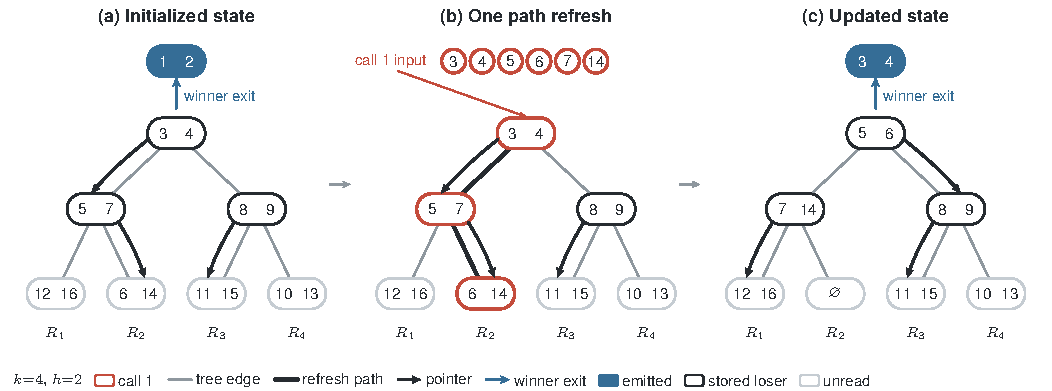
\includegraphics[width=\textwidth]{lt-h-main.pdf}
  \caption{Pointer-guided LT($h$) on the shared 16-element runs
  ($k{=}4$, $h{=}2$).
  (a)~After initialization the winner $[1,2]$ has left the root.
  Each internal node stores a loser segment and one child pointer.
  (b)~Those pointers select $R_2$.
  One \textsc{ListwiseRank} takes $[3,4,5,6,7,14]$.
  The right subtree is outside the call.
  (c)~$[3,4]$ is emitted.
  The root and the left node store the losers returned by that call,
  and their pointers are the child ids the replay returned.
  $h{=}1$ is the same generator with a shorter segment.
  The node-replay order is not expanded in this figure.}
  \label{fig:eg:loser_tree_kway_group_merge}
\end{figure*}
